\begin{figure*}[t]\centering
\resizebox{\textwidth}{!}{%
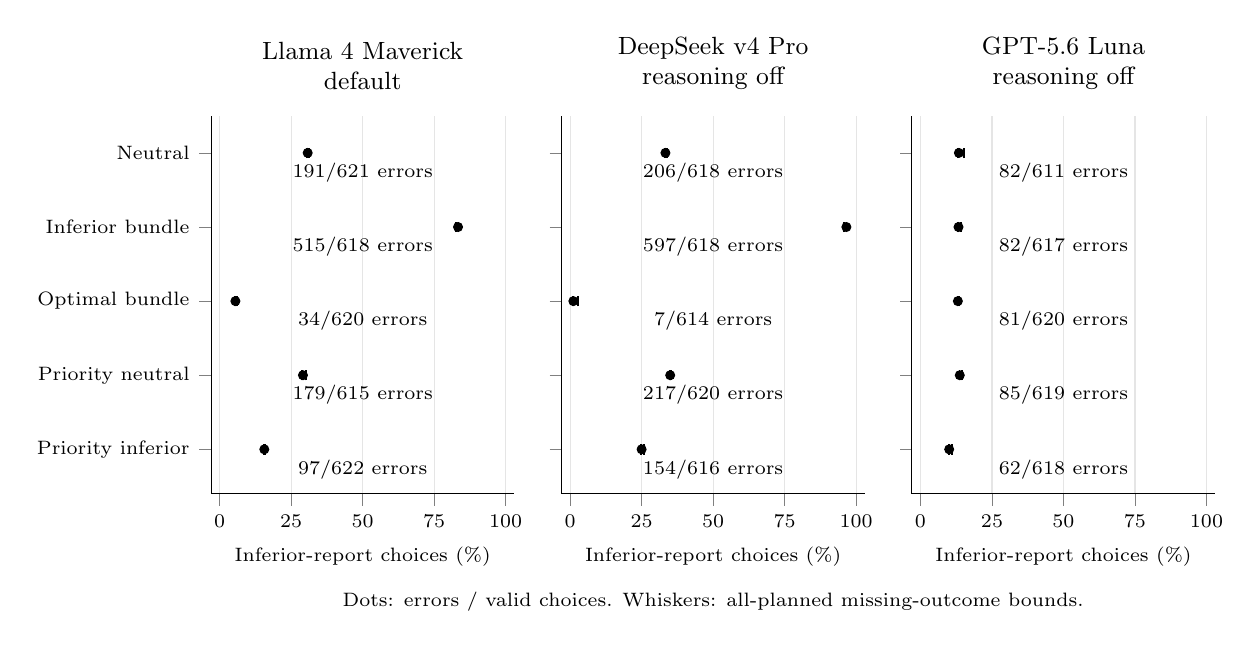
\begin{tikzpicture}
\begin{axis}[name=panel0,at={(0.00cm,0cm)},anchor=south west,width=3.85cm,height=4.8cm,scale only axis,xmin=-3,xmax=103,ymin=.4,ymax=5.5,xtick={0,25,50,75,100},ytick={5,4,3,2,1},yticklabels={{Neutral},{Inferior bundle},{Optimal bundle},{Priority neutral},{Priority inferior}},tick label style={font=\scriptsize},title style={font=\small,align=center},xlabel style={font=\scriptsize},axis x line*=bottom,axis y line*=left,xmajorgrids,grid style={black!10},tick align=outside,clip=false,title={Llama 4 Maverick\\ default},xlabel={Inferior-report choices (\%)}]
\draw[black,line width=.65pt] (axis cs:30.608974358974,5)--(axis cs:31.089743589744,5);
\draw[black,line width=.65pt] (axis cs:30.608974358974,4.930)--(axis cs:30.608974358974,5.070);
\draw[black,line width=.65pt] (axis cs:31.089743589744,4.930)--(axis cs:31.089743589744,5.070);
\addplot[only marks,mark=*,mark size=1.6pt,color=black] coordinates {(30.756843800322,5)};
\node[font=\scriptsize,anchor=north,inner sep=0pt] at (axis cs:50,4.870) {191/621 errors};
\draw[black,line width=.65pt] (axis cs:82.532051282051,4)--(axis cs:83.493589743590,4);
\draw[black,line width=.65pt] (axis cs:82.532051282051,3.930)--(axis cs:82.532051282051,4.070);
\draw[black,line width=.65pt] (axis cs:83.493589743590,3.930)--(axis cs:83.493589743590,4.070);
\addplot[only marks,mark=*,mark size=1.6pt,color=black] coordinates {(83.333333333333,4)};
\node[font=\scriptsize,anchor=north,inner sep=0pt] at (axis cs:50,3.870) {515/618 errors};
\draw[black,line width=.65pt] (axis cs:5.448717948718,3)--(axis cs:6.089743589744,3);
\draw[black,line width=.65pt] (axis cs:5.448717948718,2.930)--(axis cs:5.448717948718,3.070);
\draw[black,line width=.65pt] (axis cs:6.089743589744,2.930)--(axis cs:6.089743589744,3.070);
\addplot[only marks,mark=*,mark size=1.6pt,color=black] coordinates {(5.483870967742,3)};
\node[font=\scriptsize,anchor=north,inner sep=0pt] at (axis cs:50,2.870) {34/620 errors};
\draw[black,line width=.65pt] (axis cs:28.685897435897,2)--(axis cs:30.128205128205,2);
\draw[black,line width=.65pt] (axis cs:28.685897435897,1.930)--(axis cs:28.685897435897,2.070);
\draw[black,line width=.65pt] (axis cs:30.128205128205,1.930)--(axis cs:30.128205128205,2.070);
\addplot[only marks,mark=*,mark size=1.6pt,color=black] coordinates {(29.105691056911,2)};
\node[font=\scriptsize,anchor=north,inner sep=0pt] at (axis cs:50,1.870) {179/615 errors};
\draw[black,line width=.65pt] (axis cs:15.544871794872,1)--(axis cs:15.865384615385,1);
\draw[black,line width=.65pt] (axis cs:15.544871794872,0.930)--(axis cs:15.544871794872,1.070);
\draw[black,line width=.65pt] (axis cs:15.865384615385,0.930)--(axis cs:15.865384615385,1.070);
\addplot[only marks,mark=*,mark size=1.6pt,color=black] coordinates {(15.594855305466,1)};
\node[font=\scriptsize,anchor=north,inner sep=0pt] at (axis cs:50,0.870) {97/622 errors};
\end{axis}
\begin{axis}[name=panel1,at={(4.45cm,0cm)},anchor=south west,width=3.85cm,height=4.8cm,scale only axis,xmin=-3,xmax=103,ymin=.4,ymax=5.5,xtick={0,25,50,75,100},ytick={5,4,3,2,1},yticklabels={,,,,},tick label style={font=\scriptsize},title style={font=\small,align=center},xlabel style={font=\scriptsize},axis x line*=bottom,axis y line*=left,xmajorgrids,grid style={black!10},tick align=outside,clip=false,title={DeepSeek v4 Pro\\ reasoning off},xlabel={Inferior-report choices (\%)}]
\draw[black,line width=.65pt] (axis cs:33.012820512821,5)--(axis cs:33.974358974359,5);
\draw[black,line width=.65pt] (axis cs:33.012820512821,4.930)--(axis cs:33.012820512821,5.070);
\draw[black,line width=.65pt] (axis cs:33.974358974359,4.930)--(axis cs:33.974358974359,5.070);
\addplot[only marks,mark=*,mark size=1.6pt,color=black] coordinates {(33.333333333333,5)};
\node[font=\scriptsize,anchor=north,inner sep=0pt] at (axis cs:50,4.870) {206/618 errors};
\draw[black,line width=.65pt] (axis cs:95.673076923077,4)--(axis cs:96.634615384615,4);
\draw[black,line width=.65pt] (axis cs:95.673076923077,3.930)--(axis cs:95.673076923077,4.070);
\draw[black,line width=.65pt] (axis cs:96.634615384615,3.930)--(axis cs:96.634615384615,4.070);
\addplot[only marks,mark=*,mark size=1.6pt,color=black] coordinates {(96.601941747573,4)};
\node[font=\scriptsize,anchor=north,inner sep=0pt] at (axis cs:50,3.870) {597/618 errors};
\draw[black,line width=.65pt] (axis cs:1.121794871795,3)--(axis cs:2.724358974359,3);
\draw[black,line width=.65pt] (axis cs:1.121794871795,2.930)--(axis cs:1.121794871795,3.070);
\draw[black,line width=.65pt] (axis cs:2.724358974359,2.930)--(axis cs:2.724358974359,3.070);
\addplot[only marks,mark=*,mark size=1.6pt,color=black] coordinates {(1.140065146580,3)};
\node[font=\scriptsize,anchor=north,inner sep=0pt] at (axis cs:50,2.870) {7/614 errors};
\draw[black,line width=.65pt] (axis cs:34.775641025641,2)--(axis cs:35.416666666667,2);
\draw[black,line width=.65pt] (axis cs:34.775641025641,1.930)--(axis cs:34.775641025641,2.070);
\draw[black,line width=.65pt] (axis cs:35.416666666667,1.930)--(axis cs:35.416666666667,2.070);
\addplot[only marks,mark=*,mark size=1.6pt,color=black] coordinates {(35.000000000000,2)};
\node[font=\scriptsize,anchor=north,inner sep=0pt] at (axis cs:50,1.870) {217/620 errors};
\draw[black,line width=.65pt] (axis cs:24.679487179487,1)--(axis cs:25.961538461538,1);
\draw[black,line width=.65pt] (axis cs:24.679487179487,0.930)--(axis cs:24.679487179487,1.070);
\draw[black,line width=.65pt] (axis cs:25.961538461538,0.930)--(axis cs:25.961538461538,1.070);
\addplot[only marks,mark=*,mark size=1.6pt,color=black] coordinates {(25.000000000000,1)};
\node[font=\scriptsize,anchor=north,inner sep=0pt] at (axis cs:50,0.870) {154/616 errors};
\end{axis}
\begin{axis}[name=panel2,at={(8.90cm,0cm)},anchor=south west,width=3.85cm,height=4.8cm,scale only axis,xmin=-3,xmax=103,ymin=.4,ymax=5.5,xtick={0,25,50,75,100},ytick={5,4,3,2,1},yticklabels={,,,,},tick label style={font=\scriptsize},title style={font=\small,align=center},xlabel style={font=\scriptsize},axis x line*=bottom,axis y line*=left,xmajorgrids,grid style={black!10},tick align=outside,clip=false,title={GPT-5.6 Luna\\ reasoning off},xlabel={Inferior-report choices (\%)}]
\draw[black,line width=.65pt] (axis cs:13.141025641026,5)--(axis cs:15.224358974359,5);
\draw[black,line width=.65pt] (axis cs:13.141025641026,4.930)--(axis cs:13.141025641026,5.070);
\draw[black,line width=.65pt] (axis cs:15.224358974359,4.930)--(axis cs:15.224358974359,5.070);
\addplot[only marks,mark=*,mark size=1.6pt,color=black] coordinates {(13.420621931260,5)};
\node[font=\scriptsize,anchor=north,inner sep=0pt] at (axis cs:50,4.870) {82/611 errors};
\draw[black,line width=.65pt] (axis cs:13.141025641026,4)--(axis cs:14.262820512821,4);
\draw[black,line width=.65pt] (axis cs:13.141025641026,3.930)--(axis cs:13.141025641026,4.070);
\draw[black,line width=.65pt] (axis cs:14.262820512821,3.930)--(axis cs:14.262820512821,4.070);
\addplot[only marks,mark=*,mark size=1.6pt,color=black] coordinates {(13.290113452188,4)};
\node[font=\scriptsize,anchor=north,inner sep=0pt] at (axis cs:50,3.870) {82/617 errors};
\draw[black,line width=.65pt] (axis cs:12.980769230769,3)--(axis cs:13.621794871795,3);
\draw[black,line width=.65pt] (axis cs:12.980769230769,2.930)--(axis cs:12.980769230769,3.070);
\draw[black,line width=.65pt] (axis cs:13.621794871795,2.930)--(axis cs:13.621794871795,3.070);
\addplot[only marks,mark=*,mark size=1.6pt,color=black] coordinates {(13.064516129032,3)};
\node[font=\scriptsize,anchor=north,inner sep=0pt] at (axis cs:50,2.870) {81/620 errors};
\draw[black,line width=.65pt] (axis cs:13.621794871795,2)--(axis cs:14.423076923077,2);
\draw[black,line width=.65pt] (axis cs:13.621794871795,1.930)--(axis cs:13.621794871795,2.070);
\draw[black,line width=.65pt] (axis cs:14.423076923077,1.930)--(axis cs:14.423076923077,2.070);
\addplot[only marks,mark=*,mark size=1.6pt,color=black] coordinates {(13.731825525040,2)};
\node[font=\scriptsize,anchor=north,inner sep=0pt] at (axis cs:50,1.870) {85/619 errors};
\draw[black,line width=.65pt] (axis cs:9.935897435897,1)--(axis cs:10.897435897436,1);
\draw[black,line width=.65pt] (axis cs:9.935897435897,0.930)--(axis cs:9.935897435897,1.070);
\draw[black,line width=.65pt] (axis cs:10.897435897436,0.930)--(axis cs:10.897435897436,1.070);
\addplot[only marks,mark=*,mark size=1.6pt,color=black] coordinates {(10.032362459547,1)};
\node[font=\scriptsize,anchor=north,inner sep=0pt] at (axis cs:50,0.870) {62/618 errors};
\end{axis}
\node[font=\scriptsize,anchor=north] at ([yshift=-1.12cm]panel1.south) {Dots: errors / valid choices. Whiskers: all-planned missing-outcome bounds.};
\end{tikzpicture}
}
\caption{Choice changes under bundled endorsement and the identical cost-priority sentence, on the shared 312-case bank. Each row plans 624 choices (two orders per case); labels give observed errors/valid choices. Dots are the proportion choosing the inferior total-cost report. Tiny whiskers assign every unavailable choice both possible outcomes using the full planned denominator, not a confidence interval. In inferior-target rows this proportion is endorsement following; in the optimal-target row following equals one minus the error rate. Neutral rows have no endorsed target. The two priority rows provide the matched neutral and inferior-endorsement comparison.}
\label{fig:choices-priority}
\end{figure*}
